% !TeX document-id = {2870843d-1baa-4f6a-bd0a-a5c796104a32}
% !BIB TS-program = biber
% !TeX encoding = UTF-8
% TU Delft beamer template

\documentclass{beamer}
\usepackage[english]{babel}
\usepackage{csquotes}
\usepackage{calc}
\usepackage[absolute,overlay]{textpos}
\usepackage{graphicx}
\usepackage{subfig}
\usepackage{mathtools}
\usepackage{amsfonts}
\usepackage{amsthm}
\usepackage{comment}
\usepackage{siunitx}
\usepackage{MnSymbol,wasysym}
\usepackage{array}
\usepackage{emoji}

\setemojifont{TwemojiMozilla}

\setbeamertemplate{navigation symbols}{} % remove navigation symbols
\mode<presentation>{\usetheme[verticalbar=false]{tud}}

% BIB SETTINGS
\usepackage[
    backend=biber,
    giveninits=true,
    maxnames=30,
    maxcitenames=20,
    uniquename=init,
    url=false,
    style=authoryear,
]{biblatex}
\addbibresource{bibfile.bib}
\setlength\bibitemsep{0.3cm} % space between entries in the reference list
\renewcommand{\bibfont}{\normalfont\scriptsize}
\setbeamerfont{footnote}{size=\tiny}
\renewcommand{\cite}[1]{\footnote<.->[frame]{\fullcite{#1}}}
\setlength{\TPHorizModule}{\paperwidth}
\setlength{\TPVertModule}{\paperheight}

\newcommand{\absimage}[4][0.5,0.5]{%
	\begin{textblock}{#3}%width
		[#1]% alignment anchor within image (centered by default)
		(#2)% position on the page (origin is top left)
		\includegraphics[width=#3\paperwidth]{#4}%
\end{textblock}}

\newcommand{\mininomen}[2][1]{{\let\thefootnote\relax%
	\footnotetext{\begin{tabular}{*{#1}{@{\!}>{\centering\arraybackslash}p{1em}@{\;}p{\textwidth/#1-2em}}}%
	#2\end{tabular}}}}


\title{Taller de Git}
\author{ComCom}
\institute{DC - FCEyN - UBA}

% http://latexcolor.com/
\definecolor{lightseagreen}{rgb}{0.13, 0.7, 0.67}
\definecolor{tangelo}{rgb}{0.98, 0.3, 0.0}
\definecolor{git}{rgb}{0.94, 0.309, 0.2}

\setbeamercolor{structure}{fg=lightseagreen}

\definecolor{x11gray}{rgb}{0.75, 0.75, 0.75}
\newcommand{\code}[1]{\Colorbox{x11gray}{\lstinline{#1}}}

\newenvironment{ejercicio}[1]{
% \setbeamercolor{block title}{bg=tangelo, fg=white}
\begin{exampleblock}{#1}
}{
\end{exampleblock}
}

\newenvironment{resumen}[1]{
\setbeamercolor{block title}{bg=git, fg=white}
\begin{block}{#1}
}{
\end{block}
}

\newenvironment{comando}{
\setbeamercolor{block body}{bg=git, fg=white}
\begin{block}{}
\begin{center}
\LARGE
\begin{texttt}
}{
\end{texttt}
\end{center}
\end{block}
}

\begin{document}
\begin{frame}
  \titlepage
  \begin{figure}[ht]
      \begin{center}
          
\includegraphics[height=1in]{images/logo-taller.png}
      \end{center}
  \end{figure}
\end{frame}


\begin{frame}{Motivación 1/2}

    \begin{figure}[ht]
        \begin{center}
            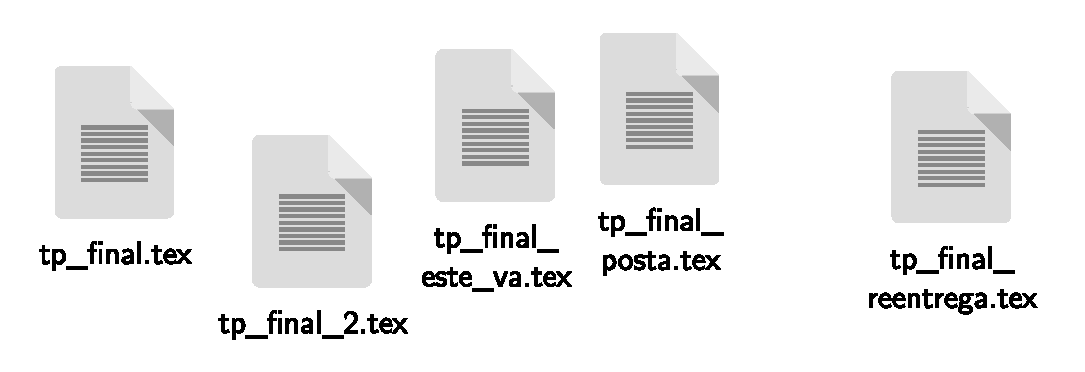
\includegraphics[height=1.5in]{images/caos.pdf}
        \end{center}
    \end{figure}

    \pause
    \begin{figure}[ht]
        \begin{center}
            
\includegraphics[height=1.5in]{images/horror.png}
        \end{center}
    \end{figure}
\end{frame}
\begin{frame}{Motivación 2/2}

    \begin{block}{Trabajando en grupo}
        \begin{itemize}
            \item Enviar cambios por mail, o
            \pause
            \item Enviar archivos por Discord, o
            \pause
            \item Sincronizar cambios por Google Docs.
        \end{itemize}
    \end{block}

    \pause
    \begin{figure}[h]
        \begin{center}
            
\includegraphics[height=1.5in]{images/horror.png}
        \end{center}
    \end{figure}

\end{frame}

\begin{frame}{¿Qué es un Sistema de Control de Versiones?}

	\begin{block}{}
 \begin{enumerate}
     \item Programas que permiten \textbf{manejar los cambios} en el código fuente de un proyecto a lo largo del tiempo.
     \item Llevan un \textbf{seguimiento} de las modificaciones que hacemos, y en caso de que nos equivoquemos, es posible volver atrás y comparar el código actual con versiones anteriores para ayudar a arreglar el error.
     \item Permiten que distintas personas modifiquen el código a la vez y \textbf{compartan los cambios}, tratando de prevenir conflictos, y en caso de que los hubiera, ayudando a identificarlos y resolverlos.
 \end{enumerate}

	\end{block}

    \pause
    \begin{resumen}{Es decir, permiten...}
        \begin{itemize}
            \item Arreglar \textit{accidentes} y volver a versiones anteriores del código.
            \item Compartir código con otras personas.
        \end{itemize}
	\end{resumen}

\end{frame}

\begin{frame}{¿Qué es Git? 1/2}

	\begin{block}{}
 \begin{itemize}
     	\item Sistema de Control de Versiones \textbf{distribuido y de código abierto}.
  
        \item Con énfasis en la \textbf{performance} (para manejar proyectos muy grandes), \textbf{seguridad} y \textbf{flexibilidad}.
        
        \item Amplio conjunto de comandos que permiten realizar operaciones de alto y bajo nivel.
 \end{itemize}

	\end{block}

    \begin{figure}[ht]
        \begin{center}
            
\includegraphics[height=1.5in]{images/logo-git.pdf}
        \end{center}
    \end{figure}
\end{frame}

\begin{frame}{¿Qué es Git? 2/2}
    \begin{center}
        \begin{block}{GIT - the stupid content tracker}

            "git" can mean anything, depending on your mood.
            
             - \textbf{random three-letter combination that is pronounceable}, and not actually used by any common UNIX command.  The fact that it is a mispronunciation of "get" may or may not be relevant.\newline
             - \textbf{stupid}. contemptible and despicable. simple. Take your pick from the dictionary of slang.\newline
             - \textbf{"global information tracker"}: you're in a good mood, and it actually works for you. Angels sing, and a light suddenly fills the room. \newline
             - \textbf{"goddamn idiotic truckload of sh*t"}: when it breaks
        \end{block}
    \end{center}
    \pause
    \textit{ - Mensaje del commit de Linus Torvalds agregando el README al repositorio Git de Git (uf)}
    
\end{frame}

\begin{frame}[t]{¿Cómo funciona Git?}
    \begin{center}
        \begin{block}{Sistema de \textit{Snapshots}}
        \begin{enumerate}
            \item Piensa a los datos como una serie de 'fotos' del sistema de archivos.
            \item Con cada commit, o cada vez que guardas el estado del repo, saca una 'foto' del mismo y guarda una referencia a esa foto.
            \item Si los archivos no cambian, no saca ninguna foto, solo mira la última.
            
        \end{enumerate}

        \end{block}

        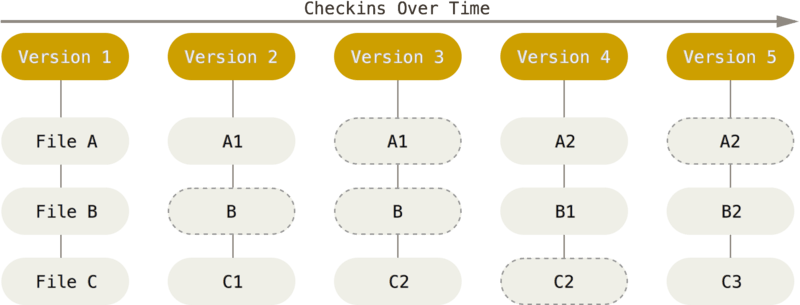
\includegraphics[width=4in]{images/snapshots.png}
    \end{center}
    
\end{frame}

\begin{frame}{Estados de un archivo}

    \begin{block}{Los cuatro estados de los archivos}
            \begin{enumerate}
    \item Untracked $\xrightarrow{}$ Sin seguimiento
    \item Unmodified $\xrightarrow{}$ Sin modificar
    \item Modified $\xrightarrow{}$ Modificado
    \item Staged, to be commited $\xrightarrow{}$ Confirmado
    \end{enumerate}
    \end{block}
    \begin{center}
        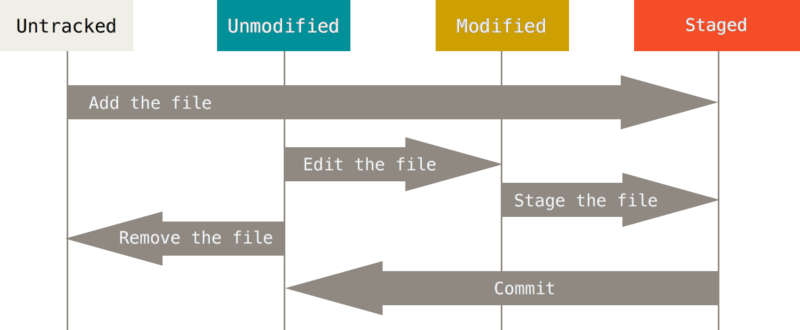
\includegraphics[width=4in]{images/lifecycle.png}
    \end{center}
    
    
\end{frame}

%pensando en sacar esta explicacion
\begin{frame}[fragile, t]{¿Está preparado, confirmado o ninguna de las dos?}
    \begin{comando}
        git status
    \end{comando}
    \pause
    \begin{block}{¡No es lo mismo!}
        Las modificaciones que hacemos pueden estar en \textbf{4 estados} distintos:
        \begin{itemize}
            \pause
            \only<-2>{\item \textbf{Sin seguimiento (untracked)}: archivos que nunca fueron agregados          al repositorio, por ejemplo archivos nuevos.}
            \only<4-4>{\item \textbf{Preparado (staged)}: las modificaciones están en \textit{staged} e
                irán en la próxima \textit{confirmación de cambios} (\textit{commit}).}
            \only<3-3>{\item \textbf{Modificado (modified)}: las modificaciones todavía no están marcadas como \textit{staged}.}
            \only<5-5>{\item \textbf{Sin modificar (unmodified)}: el estado de los archivos es el mismo que está guardado en el sistema de versionado.}
        \end{itemize}
    \end{block}

    \only<2> {
        \begin{block}{Output de ejemplo}
        \begin{center}
            \texttt{Untracked files:\\
            README}
        \end{center}
        \end{block}
    }
    \only<3> {
        \begin{block}{Output de ejemplo}
                    \begin{center}
            \texttt{Changes not staged for commit:\\
            modified: README}
        \end{center}
        \end{block}
    }
    \only<4> {
        \begin{block}{Output de ejemplo}
        \begin{center}
            \texttt{Changes to be committed:\\
            new file: README}
        \end{center}

        \end{block}
    }
    \only<5> {
        \begin{block}{Output de ejemplo}
            \begin{center}
            \texttt{nothing to commit, working directory clean}
            \end{center}
        \end{block}
    }
\end{frame}

\begin{frame}[t]{Creando un repositorio vacío}
    \begin{comando}
        git init
    \end{comando}

    \pause
    \begin{block}{}
        Crea un repositorio local vacío. Un lienzo en blanco, por así decirlo.
        \begin{enumerate}
            \item Nos paramos en el directorio que queremos convertir en un repositorio.
            \item Ejecutamos \texttt{git init}.
        \end{enumerate}
        Esto crea un subdirectorio \textit{.git} que tiene todos los archivos necesarios de Git.
    \end{block}
    \pause
    \begin{ejercicio}{Ejercicio}
        En el escritorio, creen una carpeta nueva con el nombre de su repositorio. Dentro de ella, ejecuten \texttt{git init}.
    \end{ejercicio}
\end{frame}

\begin{frame}[t]{Preparando cambios}
    \begin{comando}
        git add
    \end{comando}
    \pause
    \begin{block}{}
        Una vez que tenemos cambios hechos, tenemos que marcarlos como preparados antes de confirmarlos. En la jerga de Git, decimos que pasamos los cambios a \textit{staged}.
        \begin{enumerate}
            \item Creamos el archivo en cuestión.
            \item Ejecutamos \texttt{git add [nombre del archivo]}.
        \end{enumerate}
    \end{block}

    \pause
    \vspace{1em}
    \begin{ejercicio}{Ejercicio}
        Adentro del repositorio que crearon recién, crear un archivo y
        marcarlo como \textit{staged} usando el comando \texttt{git add}.
    \end{ejercicio}
\end{frame}

\begin{frame}{Preparando cambios (2)}
    \begin{comando}
        git add
    \end{comando}
    \begin{block}{}
        Después de modificar un archivo, tenemos que pedirle a Git que guarde su estado nuevo. 
        \begin{enumerate}
            \item Modificamos un archivo que Git marque como \texttt{modified}.
            \item Ejecutamos \texttt{git add [nombre del archivo]}
        \end{enumerate}
    \end{block}
    \pause
    \begin{ejercicio}{Ejercicio}
        Modifiquen el archivo y hagan que su estado sea \texttt{staged} de nuevo. 

        Recuerden que pueden observar los estados de los archivos con \texttt{git status}.
        
    \end{ejercicio}
    
\end{frame}

\begin{frame}[t]{Confirmando cambios}
    \begin{comando}
        git commit
    \end{comando}

    \pause
    \begin{block}{}
        Una vez que tenemos ciertos cambios en \textit{staged}, podemos confirmarlos
        ejecutando \texttt{git commit -m [mensaje]}.

        \vspace{0.5em}

        Donde \texttt{[mensaje]} es una breve descripción de los cambios que acabamos de confirmar.
    \end{block}

    \pause
    \vspace{1em}
    \pause
    \begin{ejercicio}{Ejercicio}
        Confirmar los cambios que pasaron a \textit{staged} en la diapo anterior.

        ¿Qué pasa si tienen varios archivos con distintos estados y hacen \texttt{commit}?.
    \end{ejercicio}
\end{frame}


\begin{frame}[fragile]{Configuraciones iniciales}

    \begin{block}{Tu identidad}
        Es importante establecer nuestro \textbf{nombre y email} en nuestro repositorio, ya que estos van a ir asociados con los cambios que hagamos:

        \vspace{0.5em}

        \texttt{git config --global user.name "Guybrush Threepwood"}

        \texttt{git config --global user.email guybrush@example.com}
    \end{block}
\end{frame}

\begin{frame}{Historial}
 \begin{comando}
     git log
 \end{comando}
 \pause
 \begin{block}{}
     Este comando nos sirve para ver el historial de cambios, o commits. Además nos dice quién hizo cada cosa, cuando, y su correo electrónico.
     
 \end{block}
    \begin{ejercicio}{Ejercicio}
        Fíjense quien es el autor de sus cambios anteriores...
        
        Después, hagan algún otro \texttt{commit} y miren que pasa.
    \end{ejercicio}
\end{frame}

\begin{frame}[t]{¡No seas vago con los mensajes!}

    \begin{figure}[ht]
        \begin{center}
            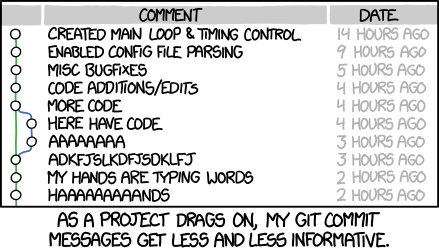
\includegraphics[height=2in]{images/xkcd-git-commit.png}
        \end{center}
        \caption{Fuente: \url{https://xkcd.com/1296/}}
    \end{figure}

\end{frame}

\begin{frame}{Colaborando con otras personas}

    Los repositorios remotos son \textit{copias} de nuestro proyecto a las cuales accedemos a través
    de Internet. Puede haber varios, cada uno de los cuales
    puede ser de solo lectura o de lectura/escritura, según los permisos que tengamos.

    \begin{figure}[ht]
        \begin{center}
            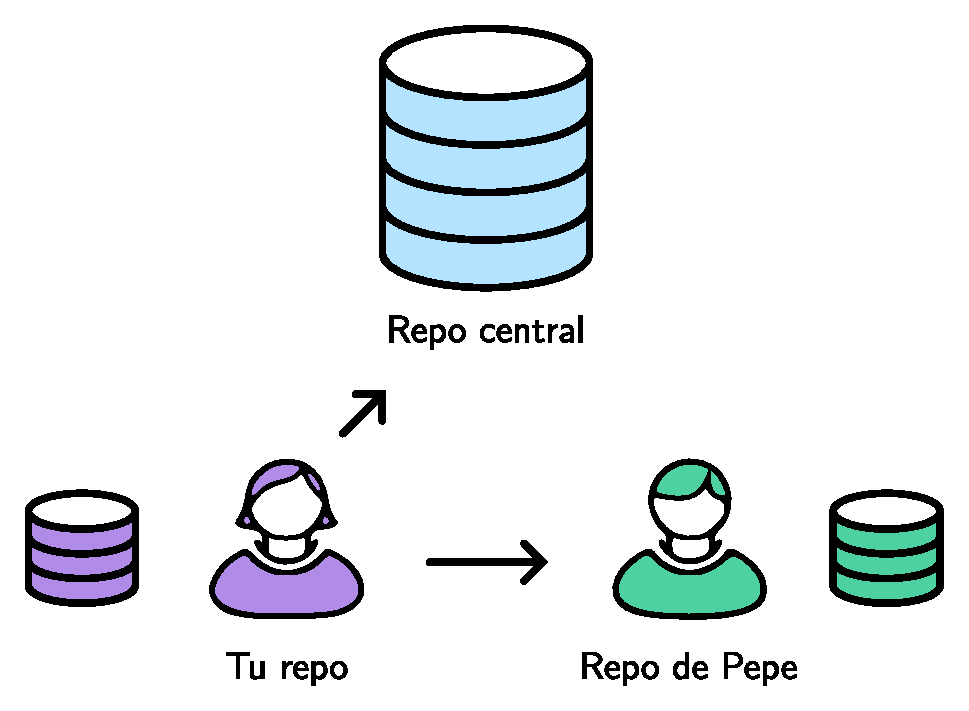
\includegraphics[height=1.5in]{images/repo-remoto.pdf}
        \end{center}
    \end{figure}

    Colaborar con otros implica gestionar estos repositorios remotos, y mandar (\textbf{push}) y recibir (\textbf{pull})
    datos de ellos cuando necesites compartir cambios.

\end{frame}

\begin{frame}{Usando Git online}
\begin{block}{Git server as a service}
    Para subir nuestros proyectos a Internet, ya sea para colaborar con otras personas o para compartir nuestro código, necesitamos usar un servicio de servidor web de Git.

    Los más conocidos son Github, SourceForge, Bitbucket y Gitlab. 
    \end{block}
    \begin{center}
        
\includegraphics[width=4in]{images/gitlab-logo-100.png}
    \end{center}

    También es posible hostear tu propia instancia de Git, por ejemplo \href{https://git.exactas.uba.ar/}{git.exactas.uba.ar}.

    
\end{frame}

\begin{frame}[t]{Enviando cambios}
    \begin{comando}
        git push
    \end{comando}

    \pause
    \begin{block}{}
        Para enviar los cambios \textbf{desde nuestro repositorio local a algún
        repositorio remoto}, ejecutamos \texttt{git push}.
    \end{block}
    \begin{ejercicio}{Ejercicio}
        Prueben hacer un push en su repo. ¿Que pasa? ¿Qué dice el error?
    \end{ejercicio}
\end{frame}

\begin{frame}[t]{Vinculando un repositorio remoto}
    \begin{comando}
        git remote
    \end{comando}

    \vspace{0.5em}
    \pause
    \begin{block}{Ver los repositorios remotos asociados}
        Ejecutamos \texttt{git remote -v}.
    \end{block}

    \pause
    \begin{block}{Agregar un repositorio remoto}
        Ejecutamos \texttt{git remote add [URL]}. %chequear esto si funciona
    \end{block}

    \begin{ejercicio}{Ejercicio}
        Agréguenle un \textit{remote} a su repo. Para esto tienen que crear un repositorio nuevo en GitLab y obtener su URL HTTPS.
    \end{ejercicio}
\end{frame}

\begin{frame}[t]{Trayendo cambios}
    \begin{comando}
        git pull
    \end{comando}

    \pause
    \begin{block}{}
        Para traer cambios \textbf{desde un repositorio remoto a nuestro repositorio local},
        ejecutamos \texttt{git pull}.

        %\vspace{0.5em}

        %Igual que antes, hasta la siguiente clase, vamos a usarlo como:\\ \texttt{git pull}.
    \end{block}
\end{frame}

\begin{frame}[t]{Obteniendo un repositorio Git}

    \begin{comando}
        git clone
    \end{comando}

    \pause
	\begin{block}{}
        Para obtener una copia local de un repositorio existente en algún servidor,
        utilizamos el comando \texttt{git clone [URL]}.
    \end{block}

    \pause
    \vspace{1em}
    \begin{ejercicio}{Ejercicio}
        \textit{Clonar} el repositorio que tiene URL: \textbf{git@gitlab.com:talleres-comcom/taller-git-ejercicio.git}
    \end{ejercicio}
\end{frame}

\begin{frame}[fragile]{Configuraciones iniciales (2)}

	\begin{block}{Clave SSH}
		Para poder trabajar cómodamente con repositorios Git que estén en Internet (GitHub, Bitbucket, GitLab, etc.), podemos configurar una \textbf{clave SSH} que nos identifique con el servidor que estemos usando.
	\end{block}

  \pause
  \begin{block}{Creando una clave nueva}
		Abrimos la terminal y ejecutamos \textit{cd~/.ssh} y luego \textit{ssh-keygen -f taller-git}. Le damos \textit{Enter} a todo.
	\end{block}

  \pause
  \begin{block}{Subiendo la clave a GitLab}
		\begin{itemize}
		\item En la terminal, ejecutamos \textit{cat taller-git.pub} y copiamos todo lo que aparezca.
      \item Abrimos GitLab, vamos a Profile Settings, SSH Keys.
      \item Pegamos lo que tenemos copiado en el campo \textit{Key}.
      \item Ponemos para que expire mañana y le damos al boton \textit{Add key}.
		\end{itemize}
	\end{block}

\end{frame}

\begin{frame}[t]{Y qué pasa si... ¡BOOM!}

    \begin{block}{A veces hay conflictos}
        \begin{itemize}
            \item Supongamos que dos personas (\emoji{penguin} y \emoji{spouting-whale}) están trabajando en un mismo proyecto.
                Es decir, ambos tienen una \textit{copia} en su máquina.
            \pause
            \item Ahora imaginemos, por ejemplo, que \emoji{penguin} modifica la línea 23 del archivo \texttt{README}
                y confirma los cambios.
            \pause
            \item Sin saberlo, \emoji{spouting-whale} también modifica la línea 23 del archivo \texttt{README}, pero pone algo distinto y confirma dichos cambios.
            \pause
            \item ¿Qué va a pasar cuando quieran compartir lo que hicieron?\\ \only<6->{\textbf{Va a haber un conflicto},
                ya que dos personas modificaron de forma distinta la misma línea.}
            \pause
            \item ¿Qué va a hacer Git?\\ \only<7->{\textbf{Se va a quejar}. A alguno de los dos le va a tocar \textbf{incorporar a mano los cambios del otro}.}
        \end{itemize}
    \end{block}

\end{frame}

\begin{frame}[t]{Apagando el incendio}

    \begin{block}{¿Cómo se ve un conflicto?}
        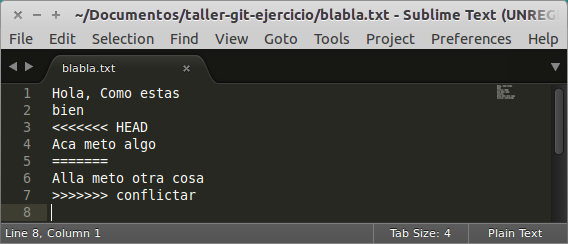
\includegraphics[height=1.0in]{images/conflicto.png}
    \end{block}

    \begin{block}{¿Qué hago?}
        \begin{itemize}
        \item Decido cómo tiene que quedar el archivo final (es decir, borro lo que quiera borrar manualmente).
        \pause
        \item Hago add.
		\pause
        \item
        Despues commit normalmente, con un mensaje como 'Merge'.
        \end{itemize}
    \end{block}

\end{frame}

\begin{frame}[t]{¡A practicar!}

    \begin{ejercicio}{Ejercicio de a 2 máquinas (preferiblemente 2 personas): \emoji{christmas-tree} y \emoji{jack-o-lantern}}
        \begin{enumerate}\begin{small}
            \pause
            \pause
            \item \emoji{christmas-tree}: crear un repositorio nuevo en \href{https://www.gitlab.com}{GitLab},
            y darle permiso a \emoji{jack-o-lantern} para hacer \textit{push}.
            \pause
            \item \emoji{christmas-tree} y \emoji{jack-o-lantern}: obtener una copia local del repositorio.
 
            \pause
            \item \emoji{christmas-tree} y \emoji{jack-o-lantern}: crear un archivo \textit{README} con contenidos distintos en la primera línea.
            \pause
            \item \emoji{christmas-tree}: hacer \textit{push} de los cambios al repositorio remoto.
            \pause
            \item \emoji{jack-o-lantern}: intentar hacer \textit{push} de los cambios al repositorio remoto. ¿Qué pasó?
            \pause
            \item \emoji{jack-o-lantern}: bajarse los cambios del repositorio remoto. ¿Anduvo?
            \pause
            \item \emoji{jack-o-lantern}: resolver los conflictos que haya.
            \pause
            \item \emoji{jack-o-lantern}: añadir y confirmar el archivo que tenía conflicto.
            \pause
            \item \emoji{jack-o-lantern}: \textit{pushear} estos nuevos cambios.
            \pause
            \item \emoji{christmas-tree}: bajarse los nuevos cambios.
        \end{small}\end{enumerate}
    \end{ejercicio}

\end{frame}

\end{document}

